\documentclass[12pt]{scrartcl}
\title{Assignment 06}
\nonstopmode
\usepackage{graphicx}
\usepackage[figurename=Figure]{caption}
\usepackage{float}
\usepackage{verbatim}
\usepackage{amsmath}
\usepackage{amssymb}
\usepackage{fullpage}
\usepackage{paralist}
\usepackage{listings}
\usepackage{subfig}
\usepackage{enumitem}
\usepackage{siunitx}
\usepackage{tikz,bm}
\usepackage{booktabs}
\usepackage{xcolor}

\definecolor{mycolor}{rgb}{1,0.2,0.3}
\definecolor{brightgreen}{rgb}{0.4, 1.0, 0.0}
\definecolor{britishracinggreen}{rgb}{0.0, 0.26, 0.15}
\definecolor{cadmiumgreen}{rgb}{0.0, 0.42, 0.24}
\definecolor{ceruleanblue}{rgb}{0.16, 0.32, 0.75}
\definecolor{darkelectricblue}{rgb}{0.33, 0.41, 0.47}
\definecolor{darkpowderblue}{rgb}{0.0, 0.2, 0.6}
\definecolor{darktangerine}{rgb}{1.0, 0.66, 0.07}
\definecolor{emerald}{rgb}{0.31, 0.78, 0.47}
\definecolor{palatinatepurple}{rgb}{0.41, 0.16, 0.38}
\definecolor{pastelviolet}{rgb}{0.8, 0.6, 0.79}

\lstset{
  basicstyle=\ttfamily\small,
  keywordstyle=\color{ceruleanblue}\bfseries,
  commentstyle=\color{cadmiumgreen},
  stringstyle=\color{mycolor},
  breaklines=true,
  frame=single,
  numbers=left,
  numberstyle=\tiny,
  language=Python
}

\begin{document}

\noindent
\begin{minipage}{0.15\textwidth}
  
\includegraphics[width=\linewidth]{logo_black.png}
\end{minipage}%
\hfill
\begin{minipage}{0.8\textwidth}
  \begin{center}
    {\textbf{\Large Indian Institute of Technology Kanpur}} \\
    \vspace{5pt}
    {\textbf{CGS698C --- Bayesian Models \& Data Analysis}}
  \end{center}
\end{minipage}

\vspace{0.4cm}
\hrule
\vspace{0.4cm}
{\hspace{-11.5pt}\textbf{Name:}\ Anandan Iyer \hspace{\fill} \textbf{Due Date:} April 17, 2026} \\
{\textbf{Roll Number:}\ 240117 \hspace{\fill} \textbf{Assignment:} 06} \\
{\textbf{Department:}\ Mechanical Engineering}\\
\hrule

% ======================================================
\section*{Part 1: Information-Theoretic Measures and Cross-Validation}

The data are 10 i.i.d.\ observations from $\text{Binomial}(20,\,\theta)$:
\[
  \mathbf{y} = \{10,15,15,14,14,14,13,11,12,16\}, \quad \sum y_i = 134, \quad \sum (20-y_i)=66.
\]

\begin{itemize}
  \item \textbf{Model 1:} $\theta \sim \text{Beta}(6,6)$
  \item \textbf{Model 2:} $\theta \sim \text{Beta}(20,60)$
\end{itemize}

Since the Beta-Binomial model is conjugate, the posterior after observing all data -
\[
  \theta \mid \mathbf{y} \sim \text{Beta}\!\left(a + \textstyle\sum y_i,\; b + \sum(n-y_i)\right).
\]

\paragraph*{Exercise 1.1} \textbf{Graph the posterior distribution of $\theta$ for each model.} \newline\newline
\textbf{Solution.}
\newline
Substituting into the conjugate update formula:

\begin{align*}
  \text{Model 1 posterior:} &\quad \theta \mid \mathbf{y} \sim \text{Beta}(6+134,\;6+66) = \text{Beta}(140,\;72), \\
  \text{Model 2 posterior:} &\quad \theta \mid \mathbf{y} \sim \text{Beta}(20+134,\;60+66) = \text{Beta}(154,\;126).
\end{align*}

The posterior means are $140/212 \approx 0.660$ and $154/280 \approx 0.550$ for Model 1 and Model 2 respectively. Model 2 is pulled toward the prior mean of $20/80=0.25$ more strongly because its prior has more pseudo-observations. Refer to the plot below.

\begin{figure}[H]
  \centering
  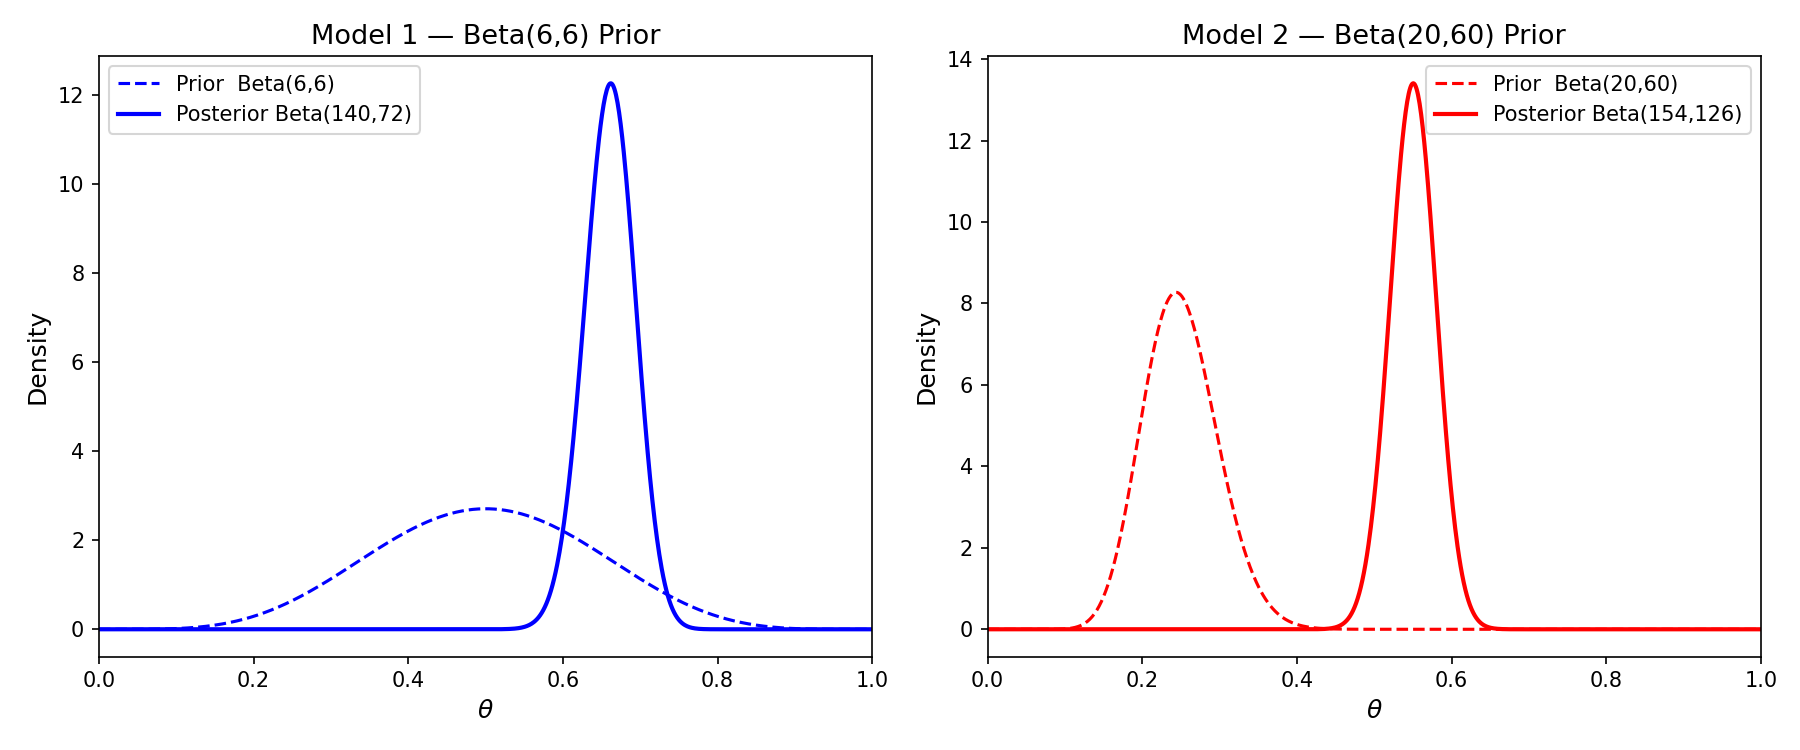
\includegraphics[width=0.92\textwidth]{posterior_plot.png}
  \caption{Prior (dashed) and posterior (solid) distributions of $\theta$ for Model 1 (left) and Model 2 (right).}
\end{figure}

\paragraph*{Exercise 1.2} \textbf{Compute log pointwise predictive density (lppd) for each model}
\newline\newline
\textbf{Solution.}

For each data point $y_i$ the log predictive density averaged over $N=10{,}000$ posterior samples is:
\[
  \ell\hat{p}d_i = \log \frac{1}{N}\sum_{j=1}^{N} p(y_i \mid \theta_j), \qquad \theta_j \sim \hat{p}(\theta \mid \mathbf{y}).
\]
The log pointwise predictive density is $\mathrm{lppd} = \sum_{i=1}^{10} \ell\hat{p}d_i$.

Table 1 reports the individual values for $\ell\hat{p}d_i$.

\begin{table}[H]
\centering
\caption{Individual $\ell\hat{p}d_i$ values for each observation.}
\label{tab:lpdi}
\begin{tabular}{cccc}
\toprule
$y_i$ & Model 1 & Model 2 \\
\midrule
10 & $-2.7726$ & $-1.8645$ \\
15 & $-1.9867$ & $-3.2375$ \\
15 & $-1.9867$ & $-3.2375$ \\
14 & $-1.7613$ & $-2.5689$ \\
14 & $-1.7613$ & $-2.5689$ \\
14 & $-1.7613$ & $-2.5689$ \\
13 & $-1.7398$ & $-2.1101$ \\
11 & $-2.2529$ & $-1.7656$ \\
12 & $-1.9069$ & $-1.8456$ \\
16 & $-2.4396$ & $-4.1397$ \\
\midrule
\textbf{lppd} & $\mathbf{-20.3691}$ & $\mathbf{-25.9072}$ \\
\bottomrule
\end{tabular}
\end{table}
\newpage
\paragraph*{Exercise 1.3} \textbf{Calculate in-sample deviance for each model from the log pointwise predictive density (lppd)
computed in Ex. 1.2.}
\\ \\
\textbf{Solution.}

$D_{\text{in}} \triangleq -2\times\mathrm{lppd}$:

\[
  D_{\text{in}}^{(1)} = -2 \times (-20.3691) = \mathbf{40.74}, \qquad
  D_{\text{in}}^{(2)} = -2 \times (-25.9072) = \mathbf{51.81}.
\]

We call this \emph{in-sample} deviance because the log predictive density is evaluated on the \emph{same} data that were used to fit (update) the posterior. The posterior already knows the data, so these log-likelihoods are biased. The model is evaluated on its training set, analogous to training-set accuracy in supervised learning.

\paragraph*{Exercise 1.4} \textbf{Based on in-sample deviance, which model is a better fit to the data?}
\\ \\ 
\textbf{Solution.}

A \emph{lower} deviance corresponds to higher predictive density and hence a better fit. Since $40.74 < 51.81$, \textbf{Model 1} has a lower in-sample deviance and fits the observed data better.

Model 2's prior places most of its mass near $\theta \approx 0.25$, which is far from the empirical rate $134/200 = 0.67$. This strongly regularises the posterior away from the data, leading to poorer fit.

\textbf{Model 1} hence fits the data better. \Box

\paragraph*{Exercise 1.5} \textbf{Suppose that you have 5 new data points: [5, 6, 10, 8, 9]. Which of your models is better at predict-
ing new data? You can calculate out-of-sample deviance now to compare your models.}
\\ \\
\textbf{Solution.}

The five new data points are $\mathbf{y}^{*} = \{5, 6, 10, 8, 9\}$. 

\[
  \mathrm{lppd}_{\text{new}}^{(1)} = -25.23, \qquad D_{\text{oos}}^{(1)} = 50.47.
\]
\[
  \mathrm{lppd}_{\text{new}}^{(2)} = -15.78, \qquad D_{\text{oos}}^{(2)} = 31.56.
\]

\textbf{Model 2} has the lower out-of-sample deviance ($31.56 < 50.47$) and therefore predicts the new data better. The new observations (mean $\approx 7.6$, empirical rate $\approx 0.38$) are much closer to the prior belief embedded in Model 2 than to Model 1's posterior mean of $0.66$. Consequently, Model 2's stronger regularization toward smaller $\theta$ generalizes better to this particular new data set.

\newpage
\paragraph*{Exercise 1.6} \textbf{Now suppose you do not have new data. Perform leave-one-out cross-validation (LOO-CV) to
compare model 1 and model 2}
\\ \\
\textbf{Solution.}

For each fold $i$, the model is fitted on the 9 remaining points and the log predictive density is evaluated on the held-out $y_i$. The LOO-CV lppd and deviance are:

\[
  \mathrm{lppd}_{\mathrm{LOO}}^{(1)} = -21.11, \qquad D_{\mathrm{LOO}}^{(1)} = 42.22.
\]
\[
  \mathrm{lppd}_{\mathrm{LOO}}^{(2)} = -27.23, \qquad D_{\mathrm{LOO}}^{(2)} = 54.46.
\]


\begin{table}[H]
\centering
\caption{LOO log predictive density for each held-out observation.}
\label{tab:loo}
\begin{tabular}{cccc}
\toprule
Fold ($y_i$ held out) & Model 1 LOO $\ell\hat{p}d_i$ & Model 2 LOO $\ell\hat{p}d_i$ \\
\midrule
10 & $-2.9989$ & $-1.8838$ \\
15 & $-2.0550$ & $-3.4691$ \\
15 & $-2.0594$ & $-3.4713$ \\
14 & $-1.7792$ & $-2.7004$ \\
14 & $-1.7769$ & $-2.7031$ \\
14 & $-1.7772$ & $-2.7021$ \\
13 & $-1.7462$ & $-2.1703$ \\
11 & $-2.3634$ & $-1.7683$ \\
12 & $-1.9500$ & $-1.8612$ \\
16 & $-2.6038$ & $-4.4996$ \\
\midrule
\textbf{LOO lppd} & $\mathbf{-21.11}$ & $\mathbf{-27.23}$ \\
\textbf{LOO deviance} & $\mathbf{42.22}$ & $\mathbf{54.46}$ \\
\bottomrule
\end{tabular}
\end{table}

Based on LOO-CV, \textbf{Model 1} has the lower LOO deviance and is the preferred model for predicting new data drawn from the same distribution as the training set.
\newpage
% ======================================================
\section*{Part 2: Marginal Likelihood and Prior Sensitivity}

Consider $k=2$ successes in $n=10$ Bernoulli trials. The marginal likelihood for a Beta$(a,b)$ prior is:
\[
  p(k \mid n, a, b) = \binom{n}{k}\frac{B(k+a,\; n-k+b)}{B(a,b)},
\]
where $B(\cdot,\cdot)$ is the Beta function.

\paragraph*{Exercise 2.1} \textbf{For $k=2$ and $n=10$, calculate marginal likelihood of the models having following priors on θ:}\\
– Beta(0.1, 0.4)\\
– Beta(1, 1)\\
– Beta(2, 6)\\
– Beta(6, 2)\\
– Beta(20, 60)\\
– Beta(60, 20)\\ \\
\textbf{Solution.}

\begin{lstlisting}[language=R, caption=Calculating Marginal Likelihood for Bernoulli Trials]
ML_binomial <- function(k,n,a,b){
ML <- (factorial(n)/(factorial(k)*factorial(n-k)))*(
factorial(k+a-1)*factorial(n-k+b-1)/factorial(n+a+b-1))
ML
}
\end{lstlisting}

\begin{table}[H]
\centering
\caption{Marginal Likelihood $p(k=2 \mid n=10)$ for various Beta priors.}
\label{tab:ml}
\begin{tabular}{lcc}
\toprule
Prior $\theta \sim $ & Marginal Likelihood (Analytical) \\
\midrule
Beta(0.1, 0.4) & 0.039809 \\
Beta(1, 1)     & 0.090909 \\
Beta(2, 6)     & 0.198529 \\
Beta(6, 2)     & 0.009718 \\
Beta(20, 60)   & 0.269359 \\
Beta(60, 20)   & 0.000799 \\
\bottomrule
\end{tabular}
\end{table}

The marginal likelihood is highest for Beta(20,60) and lowest for Beta(60,20). This reflects \textit{prior sensitivity}

\paragraph*{Exercise 2.2} \textbf{Estimate the marginal likelihood of the model given the above prior assumptions using Monte
Carlo Integration method.}
\\ \\
\textbf{Solution.}

The marginal likelihood can be written as an expectation over the prior:
\[
  p(k \mid n) = \mathbb{E}_{\theta \sim \text{Beta}(a,b)}\!\left[p(k \mid n, \theta)\right] \approx \frac{1}{M}\sum_{j=1}^{M} p(k \mid n, \theta_j), \quad \theta_j \overset{\text{iid}}{\sim} \text{Beta}(a,b).
\]

Using $M = 100{,}000$ samples the Monte Carlo estimates are given in the final column of Table~\ref{tab:ml}. All MC estimates agree with the analytical values to at least four significant figures, confirming that the Monte Carlo approximation is reliable for this problem.

\begin{table}[H]
\centering
\caption{Monte Carlo Integration Estimation $p(k=2 \mid n=10)$ for various Beta priors.}
\label{tab:ml}
\begin{tabular}{lcc}
\toprule
Prior $\theta \sim $ & Marginal Likelihood (Analytical) & MC Estimate \\
\midrule
Beta(0.1, 0.4) & 0.039809 & 0.039957 \\
Beta(1, 1)     & 0.090909 & 0.090700 \\
Beta(2, 6)     & 0.198529 & 0.198343 \\
Beta(6, 2)     & 0.009718 & 0.009731 \\
Beta(20, 60)   & 0.269359 & 0.269208 \\
Beta(60, 20)   & 0.000799 & 0.000796 \\
\bottomrule
\end{tabular}
\end{table}

\end{document}